
\chapter{INTRODUCTION}
\section{Harmful Algal Blooms}

% Introduction
Indisputably, water quality needs protection as water is essential for all life on Earth. One of the major threats to water quality is the ongoing onslaught of \gls{hab}, a disastrous phenomenon which have impacted multiple areas around the world. With \gls{hab}, algae and cyanobacteria can grow out of control, often ``painting'' the water green. \gls{hab} are a result of over-productivity of phytoplankton biomass which mostly resides near-shore in the epipelagic zone often forming a thick layer \cite{moore_richard_cyanobacterial_1993}.  \gls{hab} are dangerous due to the ecological damage from its rapid growth and the toxins they create. Unfortunately, the intensity, extent, and spatial coverage of \gls{hab} has been increasing globally due to more ecological disturbances \cite{codd_cyanobacterial_1999}. In most cases, \gls{hab} are found in coastal regions, streams, and freshwater lakes \cite{rastogi_cyanotoxin-microcystins:_2014}. \gls{hab} is a broad term which includes a large variation of different generas, depending on the location and which effected water body. The composition of \gls{hab} are diverse ranging from  different species of cyanobacteria, diatoms, algae, and dinoflagellates found worldwide \cite{dittmann_cyanobacterial_2012}. In the context of this paper, we focus on \gls{hab} that affects freshwater systems, more specifically in the state of Michigan.

% Regulations
\gls{hab} has become a national concern due to the multiple implications it poses and their occurrences. One of the dangerous qualities of \gls{hab} are the toxin compounds that are released. Cyanobacterial toxins (cyanotoxins) are diverse as over 600 peptides have been discovered \cite{welker_cyanobacterial_2006}. In response to their occurrences, the \gls{habhrca} of 2014, originally enacted in 1998, requires national programs to research and monitor \gls{hab} and to mitigate the harmful effects \cite{noauthor_harmful_2014}. The \gls{ccl} required by the \gls{sdwa} has listed cyanobacteria and cyanotoxins to be investigated by the \gls{epa} for potential future regulations \cite{usepa_drinking_2016}. 

% Toxins
One of the most prevalent toxin, \gls{mc}, is a small cyclic peptide having a large range of different structure. The mode of toxicity is its ability to inhibit protein phosphatases 1, 2A and 3 \cite{moore_richard_cyanobacterial_1993}. MC is produced mostly within the \emph{Microcystis} genera but also by other generas such as \emph{Anabaenopsis,  Nostoc,} and \emph{Planktrothrix} \cite{rastogi_cyanotoxin-microcystins:_2014, davis_phylogenies_2014}. For \gls{mc}, the \gls{who} have a guidance level of 1 $\mu$g/L for drinking water and 20 $\mu$g/L for recreational water \cite{noauthor_guidelines_1998,noauthor_guidelines_2003}. The \gls{epa} recently announced a new drinking water \gls{ha} for \gls{mc} with a guidance level of 4 $\mu$g/L for recreational surface water \cite{usepa_draft_2016}. Methods of quantifying MC will often measure \gls{mclr}. Levels above those guidelines requires state officials to issue a public health advisory not to swim in the effected area.  The common routine methods employed by state agencies are ADDA-ELISA kits by Abraxxis LLC. \gls{elisa} is an antibody method that detects and measures the ADDA-moiety of the MC. The test kit has good cross-reactivity with other congeners, and it use \gls{mclr} for its calibration standards so the reported value is in terms of MC-LR equivalence. 
Cylindrospermonsin, also under the new drinking water draft \gls{ha} \cite{usepa_draft_2016}.
Another dangerous group are called saxitoxins and are sodium channel blockers, a potent neurotoxin which paralyze and lead to death by respiratory failure \cite{moore_richard_cyanobacterial_1993}.  Anatoxins are also very dangerous exhibiting potent toxicity. It is known as Very Fast Death Factor due to its ability to irreversibly bind to nicotinic acetylcholine receptors which consequently leading to respiratory failure in a very quick manner \cite{codd_cyanobacterial_1999, moore_richard_cyanobacterial_1993}. 

Cylindrospermopsis,

% TODO need pictures of different genera of cyanos
% Toxicity
The variety of toxins have a range of different toxicity mechanisms.   %Microcystin synthesis
Microcystins are uniquely synthesized in cyanobacteria by a mix of two systems, \gls{pks} and  \gls{nrps} \cite{tillett_structural_2000}. This is different from how other proteins are normally synthesized ribosomally . The genetic mechanism of MC synthesis involves multiple protein modules spanning a 48 kilobase pair gene cluster which are responsible for incorporating different amino acids, ultimately creating the cyclic peptide \cite{moffitt_characterization_2004,nishizawa_genetic_1999}. The major amino residues of MC  are of \gls{dmeasp}, \gls{adda},  \gls{mdha} and other possible variable amino acids \cite{trogen_conformational_1996,nishizawa_genetic_1999}.
% TODO Adda group toxicity

% Microcystin congener
There are over 100 known variants of congeners of MC with 6 congeners recognized by the \gls{epa} as chemical contaminants which are \gls{mcla}, \gls{mclf}, \gls{mclr}, \gls{mcly}, \gls{mcrr}, and \gls{mcyr} \cite{puddick_modulation_2016}. The most frequently occurring and potent congener variant of MC is MC-LR \cite{rastogi_cyanotoxin-microcystins:_2014}. Figure \ref{fig:structure1} shows the structure of MC-LR which contains L-luecine (L) and L-Arginine (R) in its variable positions. Other amino acids such as alanine (A), tryptophan (W), tyrosine (Y), and phenylalanine (F) can be substituted for other variable congeners. With the known variants, MC is roughly around 1000 Da \cite{dittmann_cyanobacterial_2012}

% Ecological Damage
The harm caused by \gls{hab} does not necessarily come entirely from the toxins. In cases of \gls{hab} where there has been a large accumulation biomass, they can quickly die off due to limiting resources and cause eutrophication \cite{charlton_oxygen_1980}. The dead biomass is quickly consumed by other aquatic microorganisms which increases respiration rates, depletes dissolved oxygen creating an unsuitable habitat for other aquatic organisms.  \cite{anderson_harmful_2002}. The layer of scum formed from \gls{hab} also block light for submerged aquatic macrophytes, killing them by preventing photosythesis \cite{ bucak_modeling_2018}. \gls{hab} can also be a major nuisance and a cost to the community, as this create odor and limit recreation \cite{graham_cyanotoxin_2010, carmichael_health_2016}.


\begin{figure}[t]
   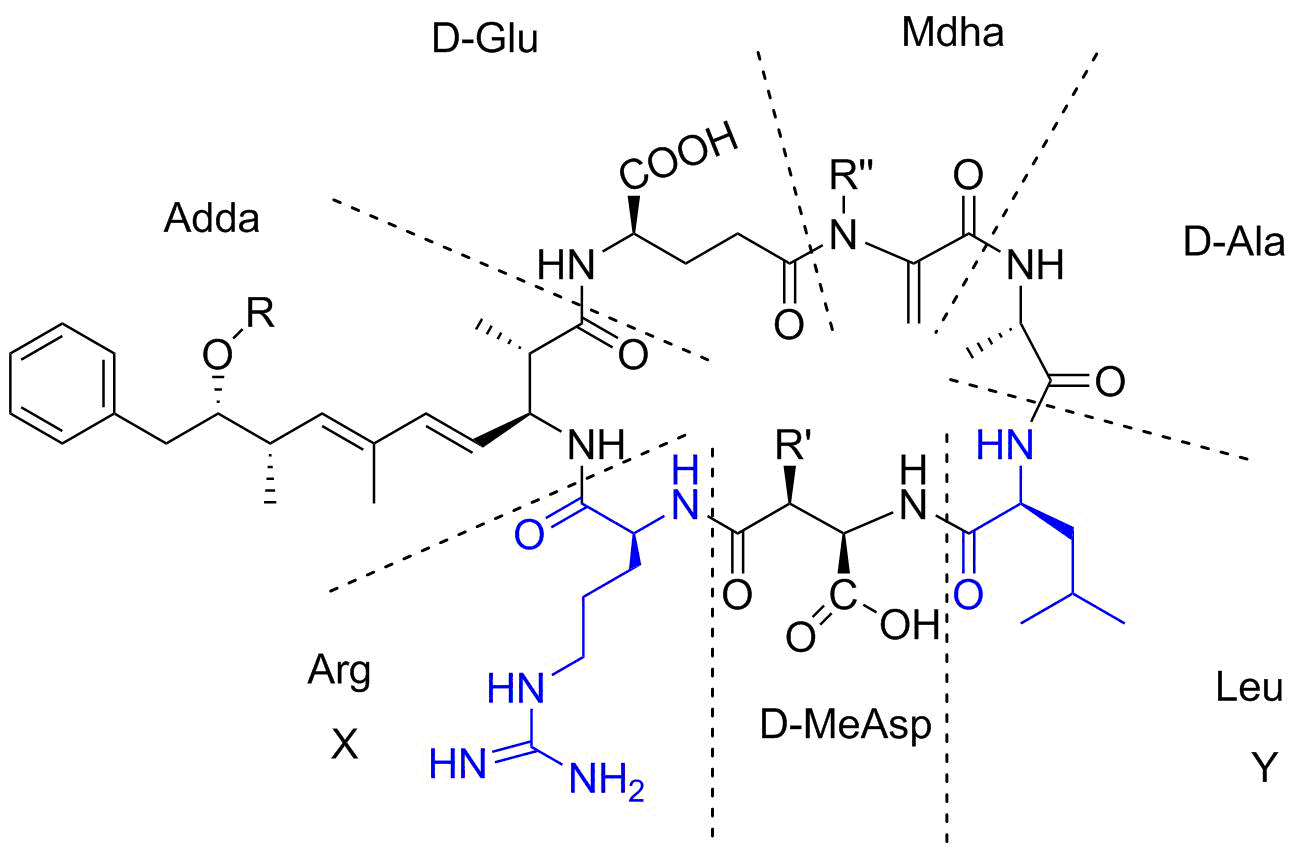
\includegraphics[width=\textwidth]{Microcystin-LR.png}
   \caption{Structure of MC-LR}
   \label{fig:structure1}
   \begin{flushleft}
   The most common structure of Microcystin. The seven amino acids are seperated by dashed lines. 
     \end{flushleft}
 \end{figure}

\section{Environmental Exposure}
% Damages
Swimming or contact in any waterbody with \gls{hab} can pose a health risk as all \gls{hab} are irritants and some can have toxin producing species. Many of the species that are producing hepatotoxins and neurotoxins in high amounts can kill livestock, pets and wildlife \cite{anderson_harmful_2002}. The possible route of exposure  for humans can be from dermal contact, accidental ingestion, breathing in lake spray aerosols and failure of purification in drinking water plants \cite{may_aerosol_2018,codd_cyanobacterial_1999}. As stated, exposure through dermal contact can be an irritant. \gls{hab} can create lipopolysaccharide, an endotoxin, which create rashes after skin contact as it triggers a inflammatory response \cite{ moore_richard_cyanobacterial_1993}.

% Treatment
Although a rare case, accidental ingestion of cyanotoxin by directly drinking water from an affected lake could  lead to acute toxicity or other symptoms \cite{monks_potent_2007}. Unfortunately, \gls{hab} can be found in storage reservoirs and source waters in regions that do not have sophisticated drinking water facilities in providing clean water. In addressing the removal of toxins, a water treatment facility needs to understand where most of the toxins resides.Cyanotoxins are mostly intracellular, except for the case of cylindrospermonspin \cite{rastogi_cyanotoxin-microcystins:_2014}.
 With a health risk management plan, an analysis of water input (raw water) needs to identify the genera and the toxins levels intracellular and extracellular concentrations \cite{saoudi_management_2017}. The information of whether the toxin is intact within the cell or not can suggest different treatments. Intact cells should be removed as much as possible at the intake without cell lysis \cite{westrick_review_2010}. Different treatment can be used with ozone, chlorination, activated carbon and advance oxidation process \cite{koreiviene_cyanotoxin_2014, westrick_cyanotoxin_2018}. However ozone and chlorination carries risk of cell lysis and disinfection by-products. The use of activated carbon or membrane filteration is effective but costly to implement as a routine \cite{koreiviene_cyanotoxin_2014}. Removal of toxins can be treated by oxidants such as \ch{KMnO4} which oxidizes the dissolved toxins and prevent the cells to lyse \cite{westrick_cyanotoxin_2018}. An effective health risk managment plan would implement a multipoint check system in the water treatment process and also be economically viable \cite{westrick_review_2010,saoudi_management_2017}.

\section{Predicting Harmful Algal Blooms}
% Drivers
The mechanism for what drives the proliferation is not fully understood \cite{dittmann_cyanobacterial_2012}. As autotrophs, \gls{hab} can rapidly grow under warm and nutrient-rich conditions \cite{rastogi_cyanotoxin-microcystins:_2014}. \gls{hab} are most likely to occur in the summer or warmer months where primary productivity is most likely to peak due to increase daylight, warmer temperature and low water flow in streams and rivers \cite{vannote_river_1980,chapra_climate_2017-2}
% Some cyanos are nitrogen fixators, succession of nitrogen to microcystin..etc
Excess nutrients, especially phosphorus is one of the most prevalent cause of \gls{hab}. %TODO citation
Urbanization and agriculture has increased the frequency of  conditions in lakes and coastal environments, often regarded as cultural eutrophication\cite{smith_eutrophication_2009}.  Organic and inorganic forms of nutrients  play a role in biomass production. Nitrogen usually from non-point sources such as septic tanks, animal waste and agricultural runoff which contributes to \gls{hab}. Phosphorus is the main culprit in freshwater in causing \gls{hab} \cite{anderson_harmful_2002}. For the bloom in Lake Erie, some studies suggests the nutrient runnoff into the  Maumee river, which has and its watershed mostly comprised of agriculture \cite{michalak_record-setting_2013, chaffin_accuracy_2018}. Other studies in other areas worldwide, similar to Lake Erie, have shown nutrient enrich conditions usually from agricultural runoff or disturbance of ecological conditions that impacts nutrient cycle to cause blooms \cite{ahn_evaluation_2011, ahn_rainfall_2002, anderson_harmful_2002, jiang_statistical_2008}.

Ecological factors could be a major factor in some cases. Previous studies in inland Michigan lakes are finding \emph{Dreissena polymorpha} (zebra mussels) to have an impact on finding blooms \cite{vanderploeg_zebra_2001}. In a study done by Michigan State University \cite{raikow_dominance_2004} found zebra mussels can promote phytoplankton growth due to their effect on bloom ecology. Some studies suggests that of zebra mussels should be incorporated in building a predictive model as they have a significant impact on \gls{hab} with their presence \cite{lavrentyev_effects_1995, knoll_invasive_2008, raikow_dominance_2004}. In our survey, we will investigate whether zebra mussels have an influence on MC concentration or cyanobacteria population.

% PREDICTIVE models
Statistical predictive models are increasingly being used to forecast \gls{hab}. Models coupled with weather data have been increasingly successful with wind direction, speed, temperature and precipitation being the best predictor of \gls{hab}. Along coastal environment,   \gls{noaa} uses real-time data from satellite to predict \gls{hab} on the Gulf of Mexico, Lake Erie, and other coastal environments based on satellite data and weather models \cite{kavanaugh_assessment_2013}. These warnings to the public can prevent exposure and improve communication with the public. They have provide effective forecast, continuously available for the public on their website \footnote{\url{https://tidesandcurrents.noaa.gov/hab_info.html}}. % TODO include phyco and chloro bouys.

Inland lakes, satellite imagery is not ideal cloudy conditions. Forecasting for inland lakes does not work with satellite imagery as the extent of the lake's area will often limit the predictability. An effective predictive models should be based on features that are found to contributes to \gls{hab} with measured abiotic and biotic factors. Understanding the main drivers for cyanobacteria can help to predict HAB occurrences.

 \section{Goals and Aims}
% TODO reread this and expand it
 One of our objectives is to have a model that is simple and robust in predicting \gls{hab}.  
My goal is to explore what drives HAB development and build a predictive model based from our collected data.  With the collected observations, I investigated the best possible predictive model from our dataset. Eventually with the built model based on each lake's unique geological characteristics and be ranked by the likelihood of \gls{hab}.
Some studies build predictive models based using cyanobacterial cell count or mass, concentrations of chloraphyll-a and MC concentrations as a response variable as its most likely associated with \gls{hab} \cite{moore_richard_cyanobacterial_1993, ahn_evaluation_2011, jiang_statistical_2008, beaulieu_nutrients_2013, taranu_predicting_2017}.
%Cyanobacteria cell counts would be ideal to measure whether the lake is exhibiting a bloom.
The total MC concentration measured by \gls{lcmsms} was used as the main predictor variable of interest. The \emph{16s rRNA} gene copies measured by \gls{qpcr} was also observed as a response variables as well as this measures relatively amount cyanobacteria. In our survey on 29 inland lakes in Michigan, we seek to understand what drives \gls{hab} and build a predictive model on \gls{mc}. In addition, we also analyzed for cylindrospermopsin and anatoxin in our surveyed lakes. Before the survey, I hypothesized if the lake's watershed is more urbanized areas, I would expect higher MC concentrations. Developed land can increase nutrient runoff which can increase algal blooms. Previous studies have shown developed areas as having a major influence on the occurrence of \gls{hab} because of more possible sources like applied fertilizer or leaky septic tanks \cite{beaver_land_2014, anderson_harmful_2002}. Lakes with higher developed areas may also have a possible influence nutrient mobility, which in turn drive MC production. I expect this relationship to also be similar with total cyanobacteria measured by \gls{qpcr}. 

My research hypotheses:

\begin{enumerate}
 \item Harmful algal blooms are influenced by  developed/urban land, which can be used to predict MC concentrations
 \item Lakes with the presence of zebra mussel will have a higher concentration of MC than lakes with none found.
 \item Nutrient concentrations can be explained by land use characteristics
 \item Identify important features that influence \gls{hab}.

\end{enumerate}
